\section{Le moteur juste avant le multic\oe{}ur}
\label{sec:contexte}

\begin{resume}
Au moment d'ouvrir le chantier multic\oe{}ur, le moteur batchait d\'ej\`a les
\'evaluations par paquets de huit gr\^ace \`a un virtual loss de type Leela
Chess Zero, et la table de transposition utilisait une cl\'e s\'emantique
\code{h0}. Le d\'ebit \'etait pass\'e de 286--299 \`a 320--850 simulations par
seconde selon la position, mais l'inf\'erence occupait d\'esormais 96 \`a
99\,\% du temps. Tout le travail restant \'etait donc d'un seul c\^ot\'e de la
barri\`ere : un unique c\oe{}ur pr\'eparait les lots, s\'erie\`element, et les
lots partiels co\^utaient leur latence fixe pour moins de positions utiles.
Ce chapitre d\'ecrit cet \'etat des lieux et les contraintes qu'il impose.
\end{resume}

\subsection{Vue d'ensemble du moteur}

Le moteur se compose de quatre ensembles, repr\'esent\'es sur la
figure~\ref{fig:architecture}. Le c\oe{}ur C++ contient le plateau
(\code{Chessboard}), le g\'en\'erateur de coups, le MCTS et sa table de
transposition, ainsi que le \code{SelfPlayManager} qui fait jouer plusieurs
parties en parall\`ele. Le r\'eseau est un ResNet de 10 blocs et 128 filtres,
avec des blocs d'attention par canal (Squeeze-and-Excitation), export\'e en
ONNX et ex\'ecut\'e par ONNX Runtime. Python orchestre l'entra\^inement, les
tournois et le bot UCI. Les deux mondes communiquent par pybind11.

\begin{figure}[t]
\centering
\begin{tikzpicture}[
  font=\small,
  boite/.style={draw=bleu!60, fill=bleuclair, rounded corners=2pt,
    minimum width=2.6cm, minimum height=0.9cm, align=center},
  boiteg/.style={draw=gris!60, fill=grisfond, rounded corners=2pt,
    minimum width=2.6cm, minimum height=0.9cm, align=center},
  fleche/.style={-{Latex[length=2mm]}, draw=gris, thick}
]
\node[boiteg] (uci) at (0,3.2) {Bot UCI\\\scriptsize (Lichess)};
\node[boiteg] (selfplay) at (4.2,3.2) {Self-play\\\scriptsize (OpenMP, 8 parties)};
\node[boite] (mcts) at (2.1,1.9) {MCTS (C++)\\\scriptsize arbre, TT, virtual loss};
\node[boite] (board) at (2.1,0.6) {Chessboard (C++)\\\scriptsize coups, Zobrist, tenseurs};
\node[boiteg] (onnx) at (0,0.6) {ONNX Runtime\\\scriptsize GPU CUDA ou CPU};
\node[boiteg] (python) at (4.2,0.6) {Python\\\scriptsize entra\^inement, tournois};

\draw[fleche] (uci) -- (mcts);
\draw[fleche] (selfplay) -- (mcts);
\draw[fleche] (mcts) -- (board);
\draw[fleche] (board) -- (onnx);
\draw[fleche] (onnx) -- node[left, font=\scriptsize, xshift=-2pt] {policy, value} (mcts);
\draw[fleche] (python) -- (mcts);
\end{tikzpicture}
\caption{Architecture du moteur. Le MCTS est partag\'e par le bot UCI et le
self-play ; le chantier multic\oe{}ur ne modifie que le premier, mais les
abstractions communes (cache, r\'eservations, \'evaluateur) servent aux deux.}
\label{fig:architecture}
\end{figure}

\subsection{Le MCTS batch\'e}

Le MCTS est un PUCT classique. Pour un enfant $i$ de parent $p$, le score de
s\'election est

\begin{equation}
\text{score}(i) = \underbrace{\frac{W_i}{N_i}}_{\text{exploitation}}
+ \underbrace{c_{\text{puct}} \cdot P_i \cdot
\frac{\sqrt{N_p}}{1 + N_i + V_i}}_{\text{exploration}},
\label{eq:puct}
\end{equation}

o\`u $N_i$ est le nombre de visites termin\'ees, $W_i$ la somme des valeurs,
$P_i$ le prior du r\'eseau, $V_i$ le nombre de descentes en cours (virtual
loss) et $c_{\text{puct}} = 1{,}4$. Deux variantes locales comptent. D'abord
le \emph{First Play Urgency} : un enfant jamais visit\'e h\'erite de la valeur
du parent, diminu\'ee d'une r\'eduction proportionnelle \`a la somme des
priors visit\'es, ce qui \'evite les erreurs catastrophiques en d\'ebut
d'exploration. Ensuite l'expansion paresseuse : un n\oe{}ud ne d\'eveloppe ses
enfants qu'au moment o\`u il devient feuille, et un succ\`es de table permet
d'\'eviter compl\`etement l'appel r\'eseau.

Le virtual loss m\'erite une pr\'ecision, car c'est le m\'ecanisme qui rend le
batching possible. En s\'electionnant le m\^eme score que ci-dessus avec
$V_i > 0$ pour les n\oe{}uds d\'ej\`a emprunt\'es par une descente en cours, on
d\'ecourage naturellement les collecteurs \`a converger vers la m\^eme
feuille. Le compteur $V$ est strictement s\'epar\'e de $N$ et de $W$ : la
valeur $Q = W/N$ reste la valeur honn\^ete de la position, et seul le terme
d'exploration est affect\'e. C'est le choix de Leela Chess Zero
\cite{lc0} ; l'alternative historique de Chaslot \cite{chaslot} ajoute une
d\'efaite fictive \`a la valeur, ce qui aurait ici contamin\'e $Q$ et,
indirectement, le First Play Urgency des fr\`eres non visit\'es.

\subsection{La table de transposition \code{h0}}

La table associe \`a une position une politique l\'egale et une valeur,
calcul\'ees par le r\'eseau, afin d'\'eviter des inf\'erences redondantes. Sa
cl\'e a fait l'objet d'un chantier ind\'ependant. Le tenseur d'entr\'ee du
r\'eseau contient huit plans d'historique, les plans de r\'ep\'etition, le
compteur des cinquante coups et des drapeaux de contexte ; le hash Zobrist
seul ne repr\'esente rien de tout cela, et un succ\`es de table sur le seul
Zobrist pouvait renvoyer une politique calcul\'ee dans un autre contexte.

La politique retenue, dite \code{h0}, prot\`ege exactement les grandeurs qui
changent la valeur ou les coups l\'egaux : le compteur de la r\`egle des
cinquante coups, la cat\'egorie de r\'ep\'etition courante et le contexte
courant (droits de roque, prise en passant, trait). Un probe v\'erifie ces
champs dans un ordre fixe et classe chaque refus (\code{RULE50\_REJECT},
\code{CONTEXT\_REJECT}, \code{HISTORY\_REJECT}) pour que les campagnes
puissent les compter s\'epar\'ement. C'est cette politique qui sert de
r\'ef\'erence \`a toutes les mesures du pr\'esent rapport.

\subsection{Le batching par virtual loss gi\`a valid\'e}

Le batching a \'et\'e introduit en septembre 2026. Sa conception
\cite{batching-design} est guide\'ee par trois observations.

\begin{enumerate}[leftmargin=1.4em]
  \item La lenteur n'\'etait pas dans la g\'en\'eration de coups : le d\'ebit
  \'etait identique entre une finale \`a 14 coups l\'egaux et un milieu \`a 48.
  \item Le rem\`ede correct \'etait le virtual loss s\'epar\'e de LC0, pas la
  d\'efaite fictive de Chaslot, pour ne pas contaminer $Q$ ni le FPU.
  \item La collecte devait capturer le plateau \`a la feuille (tenseur, coups
  l\'egaux, hash) de sorte qu'aucun rejeu de chemin ne soit n\'ecessaire
  ensuite, ni pour l'expansion ni pour l'annulation du virtual loss.
\end{enumerate}

Un lot se collecte en descendant l'arbre en posant $V$ sur chaque n\oe{}ud du
chemin, en capturant les donn\'ees \`a la feuille, puis en annulant les coups
jou\'es pour revenir \`a la racine. Une seule inf\'erence \'evalue le lot, puis
chaque feuille est d\'evelopp\'ee et remont\'ee depuis la capture. Le
balayage de taille de lot sur GPU, r\'ealis\'e le 14 septembre 2026, donne la
courbe de la figure~\ref{fig:balayage} et fixe le tableau suivant pour la
position d'ouverture (700 simulations plus tard porteront des valeurs plus
\'elev\'ees, les m\'ecanismes \'etant identiques).

\begin{figure}[t]
\centering
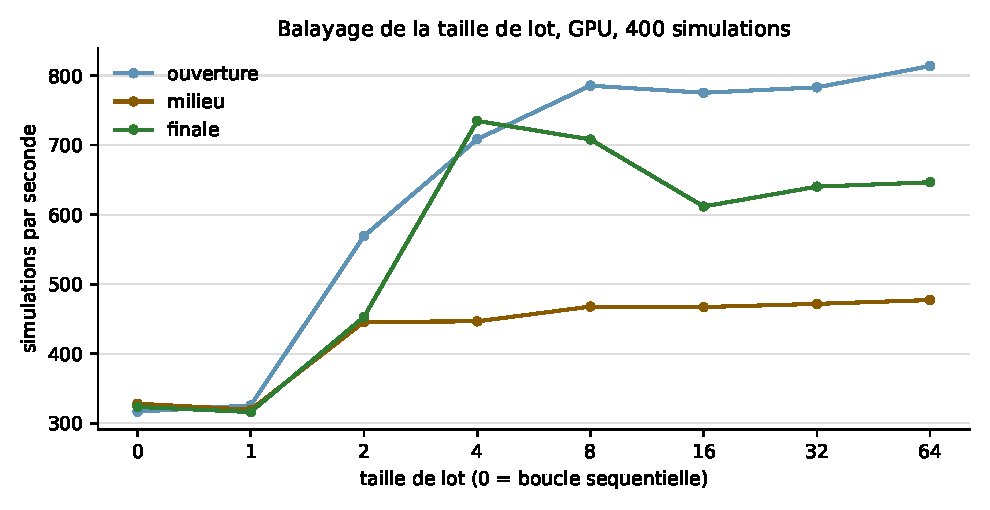
\includegraphics[width=0.78\textwidth]{figures/fig_balayage_batch.pdf}
\caption{Balayage de la taille de lot sur GPU, 400 simulations, une seule
session (donn\'ees : \code{2026-09-14-search-bench-batching-gpu.md}). Le d\'ebit
sature autour de 8 \`a 16 selon la position, et le remplissage plafonne vers
7 \`a 10 : l'arbre d'un seul arbre ne fournit pas plus de feuilles utiles.}
\label{fig:balayage}
\end{figure}

\begin{center}
\small
\begin{tabular}{lcccccc}
\toprule
Position & lot 0 & lot 2 & lot 4 & lot 8 & lot 16 & lot 64 \\
\midrule
ouverture & 316.8 & 569.2 & 708.5 & 785.5 & 775.3 & 813.7 \\
milieu    & 328.3 & 445.9 & 446.7 & 467.9 & 467.2 & 477.3 \\
finale   & 323.7 & 453.1 & 734.8 & 708.2 & 611.8 & 646.6 \\
\bottomrule
\end{tabular}
\captionof{table}{D\'ebit en simulations par seconde selon la taille de lot
(400 simulations, GPU, 5 passages). \`A lot 8, le remplissage r\'eel vaut
6,4 en ouverture, 5,0 en milieu et 5,7 en finale.}
\label{tab:balayage}
\end{center}

Le lot 8 a \'et\'e retenu : il offre presque tout le gain disponible, et sa
qualit\'e a \'et\'e valid\'ee sur 2\,500 puzzles contre le chemin s\'equentiel
(\code{batch 0} : 1\,917 r\'eussites ; \code{batch 8} : 1\,920 ; McNemar
$p = 0{,}73$, quinze paires perdues contre dix-huit gagn\'ees). Le batching
est donc actif dans le bot UCI, le jeu local et le tournoi, tandis que le
self-play, qui batchait d\'ej\`a 512 positions entre parties, n'a pas
chang\'e.

\subsection{Ce qui reste s\'eriel}

Le batching a r\'esolu le probl\`eme de la latence d'inf\'erence, mais il a
laiss\'e intacte la structure de la boucle de collecte. Cette boucle est
s\'erielle pour trois raisons pr\'ecises.

\begin{enumerate}[leftmargin=1.4em]
  \item \textbf{Un seul plateau.} La descente utilise un unique
  \code{Chessboard}, celui de l'appel. Deux descentes simultan\'ees sur le
  m\^eme plateau seraient impossibles : la g\'en\'eration des coups d\'eplace
  temporairement des pi\`eces.
  \item \textbf{Des lots partiels.} Quand une descente retombe sur une
  feuille d\'ej\`a r\'eserv\'ee, la collecte s'arr\^ete et le lot part avec
  moins de 8 positions. \`A 400 simulations, le remplissage moyen est de
  4,9 \`a 6,9 selon la position.
  \item \textbf{Des statistiques d'arbre non prot\'eg\'ees.} Visites, valeurs
  et listes d'enfants sont lues et modifi\'ees sans synchronisation adapt\'ee
  \`a plusieurs \'ecrivains concurrents.
\end{enumerate}

La cons\'equence mesur\'ee est un temps d'inactivit\'e du GPU pendant la
collecte, et un temps d'inactivit\'e du CPU pendant l'inf\'erence. Le
graphique des phases (chapitre~6) montrera que l'inf\'erence occupe 96 \`a
99\,\% du temps, et que la collecte plus les lots partiels repr\'esentent
l'essentiel du reste.

\subsection{Contraintes impos\'ees par le code}

La conception multic\oe{}ur devait composer avec six contraintes non
n\'egociables, qui expliquent la plupart des choix du chapitre suivant.

\begin{enumerate}[leftmargin=1.4em]
  \item \textbf{Un plateau complet par worker.} \code{Chessboard} n'est pas
  partageable, m\^eme pour une lecture : \code{isMoveSafe} d\'eplace et
  restaure des pi\`eces pour tester la l\'egalit\'e d'un coup. Chaque worker
  re\c{c}oit donc une copie compl\`ete du plateau (position, historiques,
  hash, tenseurs).
  \item \textbf{Un arbre unique.} Plusieurs arbres par c\oe{}ur dupliqueraient
  les \'evaluations et dilueraient la profondeur. Le b\'en\'efice de la table
  et des statistiques mutualis\'ees est le c\oe{}ur de la force du moteur, et
  \code{update\_root} r\'eutilise le sous-arbre du coup jou\'e en partie
  r\'eelle.
  \item \textbf{Une table partag\'ee.} La table doit \^etre lue et \'ecrite
  par tous les collecteurs, et par le coordinateur pendant l'expansion. Sa
  structure actuelle (un vecteur avec des pointeurs bruts) ne garantit rien.
  \item \textbf{Un self-play \`a pr\'eserver.} Le self-play utilise les m\^emes
  fonctions MCTS depuis une r\'egion OpenMP \`a huit fils, mais sur des
  parties ind\'ependantes. Ses performances et sa correction ne doivent pas
  r\'egresser.
  \item \textbf{C++17 et MSVC.} Pas de \code{std::jthread} ni de
  \code{std::barrier} : le rendez-vous des workers doit \^etre construit avec
  mutex et variables de condition. Pas de ThreadSanitizer sous MSVC : la
  correction doit reposer sur la conception et les tests, pas sur un outil
  d'analyse dynamique.
  \item \textbf{Un p\'erim\`etre fig\'e.} Les 119 plans du tenseur, le
  codage des coups, les r\`egles du plateau, la politique \code{h0}, le
  c\oe{}ur de recherche actuel \`a un worker et le self-play restent
  inchang\'es. Aucune nouvelle d\'ependance de test ni migration de langage.
\end{enumerate}

\subsection{Le cahier des charges}

La sp\'ecification de conception \cite{multicore-design} et le plan
d'impl\'ementation \cite{multicore-plan} fixent le cadre en dix t\^aches.
L'architecture cible est une recherche \emph{par vagues}, livr\'ee en deux
\'etapes compatibles : d'abord les vagues, o\`u la collecte est parall\`ele
mais le traitement est s\'equentiel apr\`es une barri\`ere ; ensuite, seulement
si les mesures le justifient, une \emph{production continue} o\`u les workers
descendent pendant les inf\'erences. La production continue n'est pas
impl\'ement\'ee ici.

Les crit\`eres d'acceptation sont explicites et seront repris au
chapitre~6 : une am\'elioration reproductible de la m\'ediane de d\'ebit, un
p95 de latence qui n'augmente pas de plus de 5\,\%, une qualit\'e de recherche
non inf\'erieure \`a 1 point de pourcentage pr\`es (bootstrap appari\'e,
marge unilat\'erale de $-1$ point), tous les invariants v\'erifi\'es et le
self-play sans r\'egression. Le r\'eglage UCI par d\'efaut ne bascule vers le
multic\oe{}ur que si tous ces crit\`eres sont franchis. Le plan prescrit un
cycle uniforme pour chaque t\^ache : \'ecrire le test en \'echec,
impl\'ementer le minimum, v\'erifier de fa\c{c}on cibl\'ee, puis commiter les
seuls fichiers concern\'es. Le chapitre~4 en raconte le d\'eroulement.

\subsection{La table du bot, rappel utile pour les mesures}

Le bot UCI construit sa table avec \code{tt\_size = 4\_000\_000} entr\'ees,
soit environ 4,16\,Gio de RAM avec la structure actuelle (1\,040 octets par
entr\'ee). Les campagnes de ce rapport utilisent une table de 8\,192 entr\'ees,
comme les bancs pr\'ec\'edents : \`a 700 simulations, elle suffit, et elle
\'elimine la variable m\'emoire des comparaisons. Cette diff\'erence est
consign\'ee comme r\'eserve au chapitre~7 : elle change le taux de succ\`es de
table en partie r\'eelle, donc l'ampleur du gain transmissible.
